\documentclass[a4paper]{article}
\usepackage[italian]{babel}
\font\TitleFont=cmr12 at 50pt
\font\AuthFont=cmr13 at 20pt
\font\ChapFont=cmr12 at 30 pt
\usepackage{titling}
\usepackage{graphicx}
\usepackage[section]{placeins}
\usepackage{tabularx}

\title {{\TitleFont Esercizio 1}}
\date{3 Luglio 2019}
\author{{\AuthFont Alessandro D'Amico}}


\renewcommand\maketitlehooka{\null\mbox{}\vfill}
\renewcommand\maketitlehookd{\vfill\null}

\begin{document}
\begin{titlingpage}
\maketitle
\end{titlingpage}
\tableofcontents
\newpage
\section{Introduzione al problema}
Nel seguente esperimento viene preso in considerazione il problema dell'ordinamento, per la cui soluzione utilizziamo due differenti algoritmi: Insertion Sort e Merge Sort.
Lo scopo e' ottenere un array (una lista di numeri) i cui elementi che lo compongono (inizialmente disposti in modo casuale) siano disposti in ordine crescente.
\section{Caratteristiche teoriche degli algoritmi utilizzati}
%devo metterle
\section{Prestazioni attese}
Un array ordinato in modo crescente rappresenta il miglior caso per Insertion Sort, mentre un array ordinato in modo decrescente rappresenta il suo caso peggiore.
\newline
\newline
	\begin{tabularx}{10cm}{|X|X|X|}
	\hline
	Algoritmo & Tempo di esecuzione caso peggiore & Tempo di esecuzione atteso / caso medio \\
	\hline
	\textbf{Insertion Sort} & $\Theta(n^2)$  & $\Theta(n^2)$ \\
	\hline
	\textbf{Merge Sort} &  $\Theta(n\log{}n)$ & $\Theta(n\log{}n)$\\
	\hline
	\end{tabularx}
\section{Esperimenti}
Sono stati effettuati i test con piu set di numeri: 
\newline
- numeri \textbf{random}
\newline 
- numeri ordinati in modo \textbf{crescente}
\newline
- numeri ordinati in modo \textbf{decrescente}
\newline
I set sono ulteriormente suddivisi in due tipologie: 
\newline
- \textbf{Small}: contengono array piccoli (fino a 200 elementi)
\newline
- \textbf{Big}: contengono array di molto grandi (fino a 100000 elementi)
\newline
\newline
Essendo difficile simulare caso migliore e peggiore di Merge Sort, ci limitiamo ad analizzare i casi peggiore, migliore e medio di Insertion Sort su entrambi gli algoritmi (il caso medio e' simulato con numeri random)
\section{Documentazione del codice}
\subsection{DataSetGenerator.py}
Questo file ha l'unica funzione di generare i Dataset.
\textbf{random\_vect(B)}: Restituisce un array di B numeri generati randomicamente (Ricevendo B in ingresso).  
\newline
\textbf{incr\_vect(B)}: Restituisce un array di B+1 numeri interi in ordine crescente e con passo 1 (da 0 a B)
\newline
\textbf{decr\_vect(B)}: Restituisce un array di B+1 numeri interi in ordine decrescente e con passo 1 (da B a 0)
\newline
\textbf{multiple\_random\_vect(MultipleNumberVect, step1, multi)}: Riceve in ingresso un array vuoto e restituisce un array di array contenenti numeri random. Gli array di numeri hanno dimensione pari al prodotto tra i e step1 dove i e' compreso tra 0 e multi.
\newline
\textbf{multiple\_incr\_vect(MultipleNumberVect, step1, multi)}: Riceve in ingresso un array vuoto e restituisce un array di array contenenti numeri ordinati in modo crescente. Gli array di numeri hanno dimensione pari al prodotto tra i e step1 dove i e' compreso tra 0 e multi. 
\newline
\textbf{multiple\_decr\_vect(MultipleNumberVect, step1, multi)}:
Riceve in ingresso un array vuoto e restituisce un array di array contenenti numeri ordinati in modo decrescente. Gli array di numeri hanno dimensione pari al prodotto tra i e step1 dove i e' compreso tra 0 e multi. 
\subsection{InsertionVsMergeBenchmark.py}
Questo file contiene il main ed i test.
\newline
\textbf{Funzioni}:
\newline
\textbf{Insertion\_sort(A)}: 
e' l'algoritmo Insertion Sort, in ingresso riceve l'array A, contenente i numeri da ordinare. Come valore di ritorno ha il tempo di esecuzione dell'algoritmo stesso.
\newline
\textbf{MergeSort(A, p, r)}:
e' l'algoritmo Merge Sort, in ingresso riceve l'array A contenente i numeri da ordinare, gli indici degli estremi dell'array da ordinare (p ed r). La funzione si chiama ricorsivamente fino ad ottenere problemi di dimensione unitaria ed in 
\newline
\textbf{Merge(A, p, q, r)}:
e' il cuore del Merge Sort (la parte "Impera").
\newline
\textbf{random\_vect(B)}: Restituisce un array di B numeri generati randomicamente (Ricevendo B in ingresso).  
\newline
\textbf{incr\_vect(B)}: Restituisce un array di B+1 numeri interi in ordine crescente e con passo 1 (da 0 a B)
\newline
\textbf{decr\_vect(B)}: Restituisce un array di B+1 numeri interi in ordine decrescente e con passo 1 (da B a 0)
\newline
\textbf{MergeSortMask(A, p, r)}: e' una chiamata a MergeSort, la sfrutto per avere un timer esterno. Il valore restituito e' il tempo d'esecuzione di Merge Sort registrato dal timer.
\newline
\textbf{testComparison(rep,Setfile)}: effettua i test sul dataset passato in ingresso Setfile ed esegue un numero di ripetizioni rep (per rendere i test indipendenti da picchi di carico del processore). Restituisce un grafico (con 2 linee) dei tempi risultanti.
\newline
\textbf{mergeTestComparison(rep)}: calcola il tempo di esecuzione di Merge Sort per ogni array di ognuno dei 3 dataset: il primo e' un dataset (di  array di varie dimensioni) di numeri random, il secondo e' un dataset (di array di varie dimensioni) di numeri ordinati in modo crescente ed il terzo e' un dataset (di array di varie dimensioni) di numeri ordinati in modo decrescente. Restituisce un grafico (con 3 linee) dei tempi risultanti.    
\newline
\textbf{insertionTestComparison(rep)}: Lo stesso di mergeTestComparison, ma con Insertion Sort.

\newpage
\section{Risultati}
\subsection{Dataset di numeri in ordine crescente}
Dalla Figura \ref{fig:SmallInsMergeCresc} traspare che per ordinare meno di 80 numeri Insertion Sort risulta piu' veloce (cio' e' dovuto principalmente al tempo impiegato al caricamento delle funzioni sulla stack).	

 
		\begin{figure}[!htb]
		\centering
		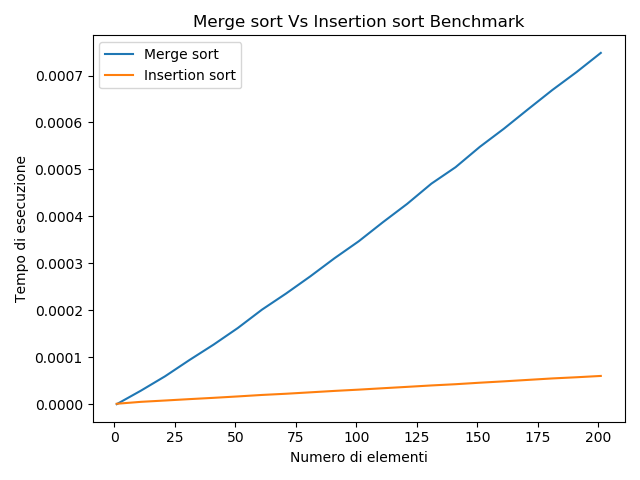
\includegraphics[scale=0.3]{2}
		\caption{Merge Sort vs Insertion Sort per pochi input (ordinati crescentemente)}
		\label{fig:SmallInsMergeCresc}
		\end{figure}
		
		\begin{figure}[!htb]
		\centering
		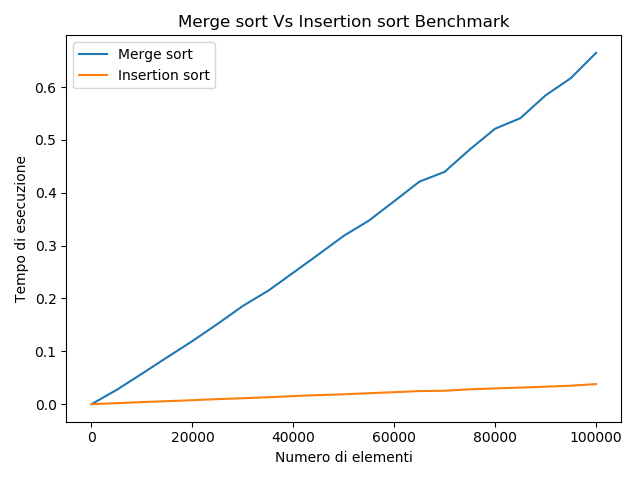
\includegraphics[scale=0.3]{1}
		\caption{Merge Sort vs Insertion Sort per molti input (ordinati crescentemente)}
		\label{fig:BigInsMergeCresc}
		\end{figure}
		

\newpage		
\subsection{Dataset di numeri in ordine decrescente}
Grazie alla figura \ref{fig:BigInsMergeDecr} e' facilmente deducibile che per grandi set di numeri da ordinare Merge Sort  e' sensibilmente piu' rapido rispetto a Insertion Sort 
 
		\begin{figure}[!htb]
		\centering
		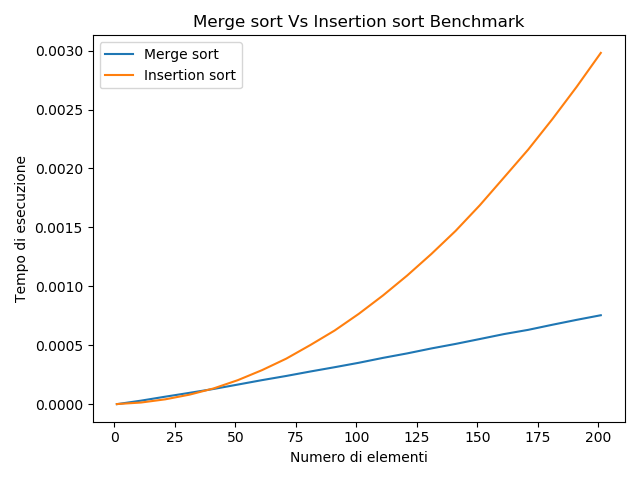
\includegraphics[scale=0.3]{4}
		\caption{Merge Sort vs Insertion Sort per pochi input (ordinati decrescentemente)}
		\label{fig:SmallInsMergeDecr}
		\end{figure}
		
		\begin{figure}[!htb]
		\centering
		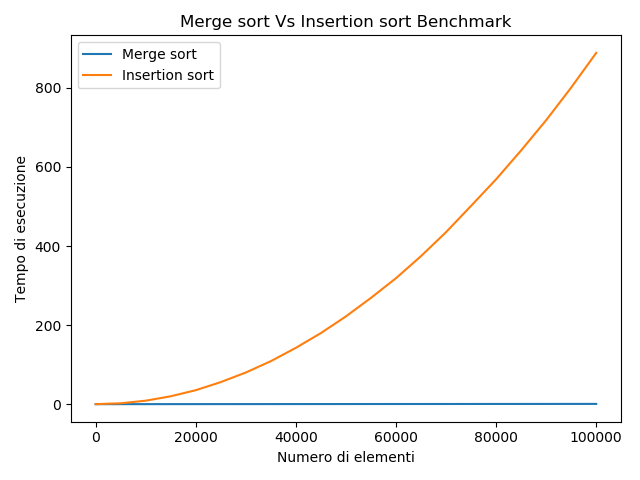
\includegraphics[scale=0.3]{3}
		\caption{Merge Sort vs Insertion Sort per molti input (ordinati decrescentemente)}
		\label{fig:BigInsMergeDecr}
		\end{figure}
\newpage		
\subsection{Dataset di numeri in ordine random}		

		\begin{figure}[!htb]
		\centering
		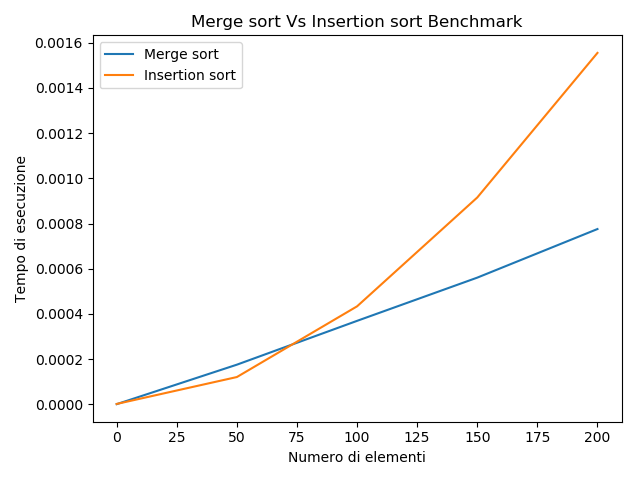
\includegraphics[scale=0.3]{6}
		\caption{Merge Sort vs Insertion Sort per pochi input (random)}
		\label{fig:SmallInsMergeRandom}
		\end{figure}
		
		\begin{figure}[!htb]
		\centering
		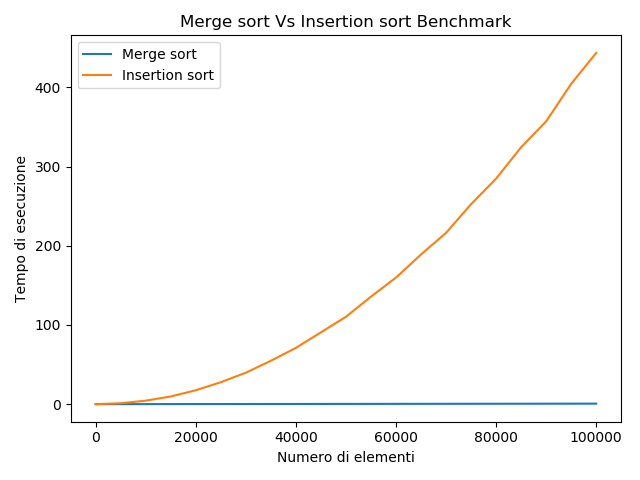
\includegraphics[scale=0.3]{5}
		\caption{Merge Sort vs Insertion Sort per molti input (random)}
		\label{fig:BigInsMergeRandom}
		\end{figure}
\newpage
\subsection{Merge Sort per dataset delle varie tipologie}
		\begin{figure}[!htb]
		\centering
		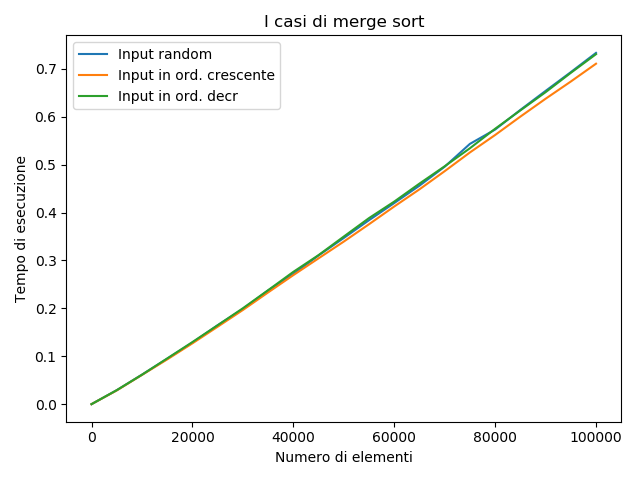
\includegraphics[scale=0.3]{CasiMerge}
		\caption{Merge Sort per varie tipologie di dataset}
		\label{fig:CasiMerge}
		\end{figure}
\subsection{Insertion Sort per dataset delle varie tipologie}
		\begin{figure}[!htb]
		\centering
		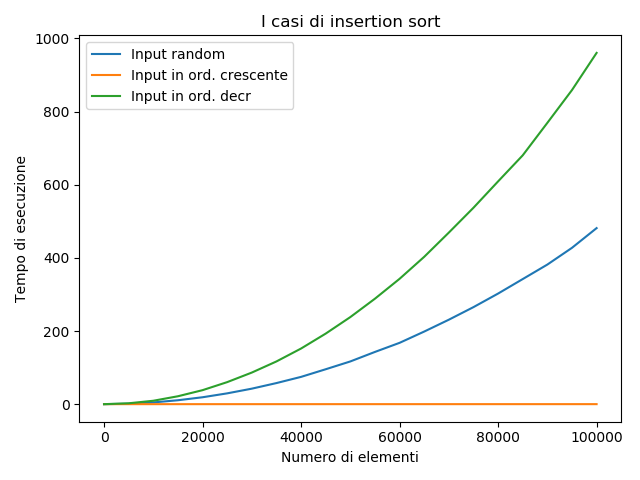
\includegraphics[scale=0.3]{CasiInsertion}
		\caption{Insertion Sort per varie tipologie di dataset}
		\label{fig:CasiInsertion}
		\end{figure}
\section{Conclusioni}
E' stato verificato il comportamento dei due algoritmi al variare della tipologia di dataset utilizzati. Possiamo concludere che per una quantita' molto ridotta di numeri da ordinare (pari a circa 80) e' conveniente utilizzare Insertion Sort (essendo Merge Sort ricorsivo, l'operazione di caricamento della funzione sulla stack richiede un tempo, che per pochi input puo' incidere sensibilmente sul tempo finale), ma escluso tale caso ed il caso in cui tutti i numeri risultino ordinati, Merge Sort risulta notevolmente piu' veloce.
\end{document}
